\documentclass{article}
\usepackage[preprint]{neurips_2024}
\usepackage[utf8]{inputenc}
\usepackage[T1]{fontenc}
\usepackage[colorlinks=true,linkcolor=black,citecolor=blue!50!black,urlcolor=blue!50!black]{hyperref}
\usepackage{url}
\usepackage{booktabs}
\usepackage{amsmath,amssymb,amsthm}
\usepackage{cancel}
\usepackage{microtype}
\usepackage{xcolor}
\usepackage{tikz}
\usetikzlibrary{arrows.meta,positioning}

\newtheorem{proposition}{Proposition}[section]
\newtheorem{lemma}[proposition]{Lemma}
\newtheorem{corollary}[proposition]{Corollary}
\theoremstyle{definition}
\newtheorem{definition}[proposition]{Definition}
\newtheorem{assumption}{Assumption}
\theoremstyle{remark}
\newtheorem{remark}[proposition]{Remark}
\newtheorem{example}[proposition]{Example}

\newcommand{\E}{\mathbb{E}}
\newcommand{\dE}{\Delta E}
\newcommand{\dP}{\Delta P}
\newcommand{\Ob}{\bar O}
\newcommand{\KL}{\mathrm{KL}}
\newcommand{\why}[1]{\tag*{\small(#1)}}

\title{The State Defect, Empowerment and Plasticity}

\author{XXX}

\begin{document}
\maketitle

\begin{abstract}
For an agent that acts on a memory, we derive the empowerment and plasticity mismatches between the history and the memory, the two splits of the state defect, and three ways to separate the reward inside them. We then follow the interaction step by step: the Bellman equation with the current action set and the later actions generated by the policy, the memory's own Bellman prediction and its error, and how an improvement of the next policy, limited by what the next memory holds, reaches the value of the current action. As preliminary results, we relate the information terms to the order of actions and to single-step improvement, and study the selection made by the agent's next action and the dependence of the memory's model on the policy. Every derivation is written term by term, and every cancellation names the assumption or lemma that allows it.
\end{abstract}

\section{Setting}\label{sec:setting}

\begin{center}
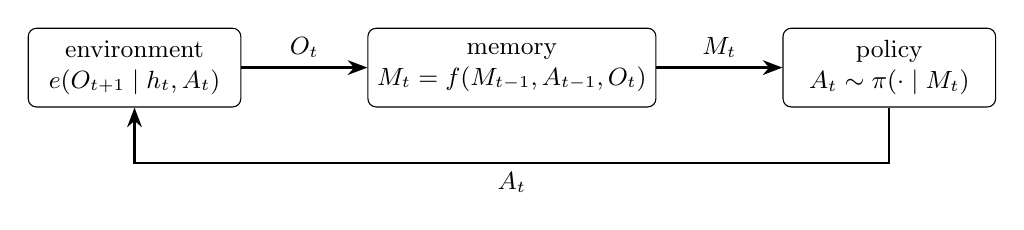
\begin{tikzpicture}[>={Stealth[length=2.5mm]}, node distance=10mm and 16mm,
  box/.style={draw, rounded corners=3pt, minimum height=10mm, minimum width=27mm, align=center, font=\small}]
\node[box] (world) {environment\\ $e(O_{t+1}\mid h_t, A_t)$};
\node[box, right=of world] (mem) {memory\\ $M_t = f(M_{t-1}, A_{t-1}, O_t)$};
\node[box, right=of mem] (pol) {policy\\ $A_t \sim \pi(\cdot \mid M_t)$};
\draw[->, thick] (world) -- node[above, font=\small] {$O_t$} (mem);
\draw[->, thick] (mem) -- node[above, font=\small] {$M_t$} (pol);
\draw[->, thick] (pol.south) -- ++(0,-7mm) -| node[pos=0.25, below, font=\small] {$A_t$} (world.south);
\end{tikzpicture}
\end{center}

The history is $h_t=(O_1,A_1,\dots,A_{t-1},O_t)$. The observation contains the reward: $O_t=(R_t,\Ob_t)$, with $\Ob_t$ the rest of the observation. All observation and action sets are finite, and all probabilities are under the law of the agent's experience induced by the three boxes.

\begin{assumption}[Environment]\label{as:env}
$O_{t+1}\sim e(\cdot\mid h_t,A_t)$ for some law $e$; the environment may depend on the whole history, with no Markov or stationarity condition.
\end{assumption}

\begin{assumption}[Memory]\label{as:mem}
$M_1=f_1(O_1)$ and $M_{t+1}=f(M_t,A_t,O_{t+1})$ for fixed maps $f_1,f$. Hence $M_t$ is a function of $h_t$.
\end{assumption}

\begin{assumption}[Policy]\label{as:pol}
$P(A_t=a\mid h_t)=\pi(a\mid M_t)$: the action depends on the history only through the memory.
\end{assumption}

Every identity in Sections~\ref{sec:setting}--\ref{sec:reward} was checked numerically, and those of Sections~\ref{sec:bellman}--\ref{sec:adapt} as described there. The script \texttt{checks/verify\_note.py} computes the exact law of all trajectories in small random environments whose next observation depends on the whole history, and tests each numbered statement for a finite horizon; the largest error is $10^{-13}$.

\section{Tools}\label{sec:tools}

We use five standard facts \citep[Ch.~2]{cover2006elements}. $X,Y,W,Z$ are random variables, and conditioning on nothing is allowed.
\begin{enumerate}
\item[(T1)] $I(X;Y\mid Z)=H(X\mid Z)-H(X\mid Y,Z)=H(Y\mid Z)-H(Y\mid X,Z)$.
\item[(T2)] Chain rule: $I(X,Y;W\mid Z)=I(X;W\mid Z)+I(Y;W\mid Z,X)=I(Y;W\mid Z)+I(X;W\mid Z,Y)$, and the same with the pair in the second place, since $I$ is symmetric.
\item[(T3)] $I(X;Y\mid Z)\ge0$, with equality exactly when $X$ and $Y$ are independent given $Z$.
\item[(T4)] If $W$ is a function of $X$, conditioning on $(X,W)$ is the same as conditioning on $X$: $H(Y\mid X,W,Z)=H(Y\mid X,Z)$. By Assumption~\ref{as:mem}, this applies to $W=M_t$, $X=h_t$.
\item[(T5)] $h_{t+1}=(h_t,A_t,O_{t+1})$, so conditioning on $h_{t+1}$ is the same as conditioning on $(h_t,A_t,O_{t+1})$.
\end{enumerate}

\begin{lemma}[The action depends on the past only through the memory]\label{lem:action}
Under Assumptions~\ref{as:mem} and~\ref{as:pol}, for every $k\ge0$,
\[
H(A_{t+k}\mid h_t,A_t,O_{t+1},\dots,A_{t+k-1},O_{t+k})=H(A_{t+k}\mid M_t,A_t,O_{t+1},\dots,A_{t+k-1},O_{t+k}),
\]
and therefore $I(h_t;A_{t+k}\mid M_t,A_t,O_{t+1},\dots,A_{t+k-1},O_{t+k})=0$. The cases used most are
\begin{align*}
\text{(a) } k=0:&\quad H(A_t\mid h_t)=H(A_t\mid M_t),\\
\text{(b) } k=1:&\quad H(A_{t+1}\mid h_t,A_t,O_{t+1})=H(A_{t+1}\mid M_t,A_t,O_{t+1}).
\end{align*}
\end{lemma}

\begin{proof}
By (T5) applied $k$ times, the conditioning variables on the left are $h_{t+k}$. By Assumption~\ref{as:pol}, the law of $A_{t+k}$ given $h_{t+k}$ is $\pi(\cdot\mid M_{t+k})$. By Assumption~\ref{as:mem}, $M_{t+k}$ is obtained from $M_t$ by applying $f$ $k$ times with the inputs $(A_t,O_{t+1}),\dots,(A_{t+k-1},O_{t+k})$, so it is a function of the conditioning variables on the right. These variables are a function of $h_{t+k}$, so the law of $A_{t+k}$ given them is the average of $\pi(\cdot\mid M_{t+k})$ over the histories consistent with them, which is $\pi(\cdot\mid M_{t+k})$ itself. Both laws are $\pi(\cdot\mid M_{t+k})$, so the two entropies are equal. For the mutual information, write $C=(A_t,O_{t+1},\dots,A_{t+k-1},O_{t+k})$ in this proof only:
\begin{align*}
I(h_t;A_{t+k}\mid M_t,C)
&=H(A_{t+k}\mid M_t,C)-H(A_{t+k}\mid h_t,M_t,C) \why{T1}\\
&=H(A_{t+k}\mid M_t,C)-H(A_{t+k}\mid h_t,C) \why{T4}\\
&=0 \why{the equality of entropies above}.
\end{align*}
\end{proof}
\section{Empowerment and plasticity at the history and at the memory}\label{sec:EP}

In every derivation below, the label at the right of a line names the fact used to obtain that line. Two struck-through terms in a line are equal by the named fact and cancel.

\begin{definition}\label{def:EP}
Following the one-step form of \citet{abel2025plasticity}, the empowerment of the action and the plasticity of the next action, computed from the history and from the memory, are
\begin{align*}
E_t&=I(A_t;O_{t+1}\mid h_t), & E_t(M)&=I(A_t;O_{t+1}\mid M_t),\\
P_{t+1}&=I(O_{t+1};A_{t+1}\mid h_t,A_t), & P_{t+1}(M)&=I(O_{t+1};A_{t+1}\mid M_t,A_t),
\end{align*}
and the two mismatches are $\dE_t=E_t-E_t(M)$ and $\dP_t=P_{t+1}(M)-P_{t+1}$.
\end{definition}

\begin{proposition}[Empowerment mismatch]\label{prop:dE}
Under Assumptions~\ref{as:mem} and~\ref{as:pol}, $\dE_t=I(h_t;A_t\mid M_t,O_{t+1})\ge0$.
\end{proposition}

\begin{proof}
Write both empowerments with (T1), with $A_t$ as the variable whose entropy is taken:
\begin{align*}
E_t&=H(A_t\mid h_t)-H(A_t\mid h_t,O_{t+1}),\\
E_t(M)&=H(A_t\mid M_t)-H(A_t\mid M_t,O_{t+1}).
\end{align*}
Subtract:
\begin{align*}
\dE_t&=\cancel{H(A_t\mid h_t)}-H(A_t\mid h_t,O_{t+1})-\cancel{H(A_t\mid M_t)}+H(A_t\mid M_t,O_{t+1}) \why{struck terms equal, Lemma~\ref{lem:action}(a)}\\
&=H(A_t\mid M_t,O_{t+1})-H(A_t\mid h_t,O_{t+1})\\
&=H(A_t\mid M_t,O_{t+1})-H(A_t\mid h_t,M_t,O_{t+1}) \why{T4}\\
&=I(h_t;A_t\mid M_t,O_{t+1}) \why{T1},
\end{align*}
which is nonnegative by (T3).
\end{proof}

\begin{proposition}[Plasticity mismatch]\label{prop:dP}
Under Assumptions~\ref{as:mem} and~\ref{as:pol}, $\dP_t=I(h_t;A_{t+1}\mid M_t,A_t)\ge0$.
\end{proposition}

\begin{proof}
Write both plasticities with (T1), with $A_{t+1}$ as the variable whose entropy is taken:
\begin{align*}
P_{t+1}&=H(A_{t+1}\mid h_t,A_t)-H(A_{t+1}\mid h_t,A_t,O_{t+1}),\\
P_{t+1}(M)&=H(A_{t+1}\mid M_t,A_t)-H(A_{t+1}\mid M_t,A_t,O_{t+1}).
\end{align*}
Subtract:
\begin{align*}
\dP_t&=H(A_{t+1}\mid M_t,A_t)-\cancel{H(A_{t+1}\mid M_t,A_t,O_{t+1})}\\
&\quad-H(A_{t+1}\mid h_t,A_t)+\cancel{H(A_{t+1}\mid h_t,A_t,O_{t+1})} \why{struck terms equal, Lemma~\ref{lem:action}(b)}\\
&=H(A_{t+1}\mid M_t,A_t)-H(A_{t+1}\mid h_t,A_t)\\
&=H(A_{t+1}\mid M_t,A_t)-H(A_{t+1}\mid h_t,M_t,A_t) \why{T4}\\
&=I(h_t;A_{t+1}\mid M_t,A_t) \why{T1},
\end{align*}
which is nonnegative by (T3).
\end{proof}

In words: given the outcome, the history still tells something about the action that the memory does not, so the memory underestimates empowerment; and the history tells something about the next action that the memory does not, so the memory overestimates plasticity.

\section{The state defect and its two splits}\label{sec:splits}

\begin{definition}\label{def:terms}
The state defect and two further terms are
\[
D_t=I(h_t;O_{t+1}\mid M_t,A_t),\qquad D^0_t=I(h_t;O_{t+1}\mid M_t),\qquad D^+_t=I(h_t;O_{t+1}\mid M_t,A_t,A_{t+1}).
\]
With Propositions~\ref{prop:dE} and~\ref{prop:dP}, each of the five terms is a mutual information between the history and one variable, given the memory and other variables:
\begin{center}
\small
\begin{tabular}{llll}
\toprule
term & mutual information & variable predicted & given, besides $M_t$\\
\midrule
$D_t$ & $I(h_t;O_{t+1}\mid M_t,A_t)$ & $O_{t+1}$ & $A_t$\\
$D^0_t$ & $I(h_t;O_{t+1}\mid M_t)$ & $O_{t+1}$ & nothing\\
$\dE_t$ & $I(h_t;A_t\mid M_t,O_{t+1})$ & $A_t$ & $O_{t+1}$\\
$\dP_t$ & $I(h_t;A_{t+1}\mid M_t,A_t)$ & $A_{t+1}$ & $A_t$\\
$D^+_t$ & $I(h_t;O_{t+1}\mid M_t,A_t,A_{t+1})$ & $O_{t+1}$ & $A_t,A_{t+1}$\\
\bottomrule
\end{tabular}
\end{center}
By (T1) and (T4), each is the uncertainty about the predicted variable given the memory minus the uncertainty given the history.
\end{definition}

\begin{proposition}[First split]\label{prop:split1}
Under Assumptions~\ref{as:mem} and~\ref{as:pol}, $D_t=D^0_t+\dE_t$.
\end{proposition}

\begin{proof}
Apply (T2) to $I(h_t,A_t;O_{t+1}\mid M_t)$ in the two orders.

History first:
\begin{align*}
I(h_t,A_t;O_{t+1}\mid M_t)&=I(h_t;O_{t+1}\mid M_t)+I(A_t;O_{t+1}\mid M_t,h_t) \why{T2}\\
&=D^0_t+I(A_t;O_{t+1}\mid h_t) \why{Definition~\ref{def:terms}; T4}\\
&=D^0_t+E_t \why{Definition~\ref{def:EP}}.
\end{align*}
Action first:
\begin{align*}
I(h_t,A_t;O_{t+1}\mid M_t)&=I(A_t;O_{t+1}\mid M_t)+I(h_t;O_{t+1}\mid M_t,A_t) \why{T2}\\
&=E_t(M)+D_t \why{Definitions~\ref{def:EP} and~\ref{def:terms}}.
\end{align*}
The two right sides are equal, so $D^0_t+E_t=E_t(M)+D_t$, that is, $D_t=D^0_t+E_t-E_t(M)=D^0_t+\dE_t$.
\end{proof}

\begin{proposition}[Second split]\label{prop:split2}
Under Assumptions~\ref{as:mem} and~\ref{as:pol}, $D_t=\dP_t+D^+_t$.
\end{proposition}

\begin{proof}
Apply (T2) to $I(h_t;O_{t+1},A_{t+1}\mid M_t,A_t)$ in the two orders.

Next observation first:
\begin{align*}
I(h_t;O_{t+1},A_{t+1}\mid M_t,A_t)&=I(h_t;O_{t+1}\mid M_t,A_t)+I(h_t;A_{t+1}\mid M_t,A_t,O_{t+1}) \why{T2}\\
&=D_t+0 \why{Definition~\ref{def:terms}; Lemma~\ref{lem:action}, $k=1$}.
\end{align*}
Next action first:
\begin{align*}
I(h_t;O_{t+1},A_{t+1}\mid M_t,A_t)&=I(h_t;A_{t+1}\mid M_t,A_t)+I(h_t;O_{t+1}\mid M_t,A_t,A_{t+1}) \why{T2}\\
&=\dP_t+D^+_t \why{Proposition~\ref{prop:dP}; Definition~\ref{def:terms}}.
\end{align*}
The two right sides are equal.
\end{proof}

\begin{remark}[Both splits come from one quantity]\label{rem:orders}
Apply (T2) to $I(h_t;A_t,O_{t+1},A_{t+1}\mid M_t)$ in three orders. In the order of time, $(A_t,O_{t+1},A_{t+1})$, the terms are $I(h_t;A_t\mid M_t)=0$ (Lemma~\ref{lem:action}, $k=0$), $D_t$, and $I(h_t;A_{t+1}\mid M_t,A_t,O_{t+1})=0$ (Lemma~\ref{lem:action}, $k=1$). In the order $(O_{t+1},A_t,A_{t+1})$ they are $D^0_t$, $\dE_t$ and $I(h_t;A_{t+1}\mid M_t,O_{t+1},A_t)=0$. In the order $(A_t,A_{t+1},O_{t+1})$ they are $0$, $\dP_t$ and $D^+_t$. So the first split reads the action $A_t$ after the observation it produced, the second reads the next action $A_{t+1}$ before the observation it responds to, and in the order of time the two actions contribute nothing.
\end{remark}

\begin{corollary}\label{cor:consequences}
Under Assumptions~\ref{as:mem} and~\ref{as:pol}:
\begin{enumerate}
\item[(a)] $D_t=0$ if and only if $D^0_t=0$ and $\dE_t=0$, and if and only if $\dP_t=0$ and $D^+_t=0$;
\item[(b)] $\dP_t\le D_t$;
\item[(c)] $\dE_t\le H(A_t\mid M_t)$, so $\dE_t=0$ and $D_t=D^0_t$ when the policy is deterministic.
\end{enumerate}
\end{corollary}

\begin{proof}
(a) Each term is nonnegative (T3), and a sum of two nonnegative terms is zero exactly when both are. (b) From Proposition~\ref{prop:split2}, since $D^+_t\ge0$. (c) $\dE_t=H(A_t\mid M_t,O_{t+1})-H(A_t\mid h_t,O_{t+1})\le H(A_t\mid M_t,O_{t+1})\le H(A_t\mid M_t)$, where the first step drops a nonnegative entropy and the second uses that conditioning does not increase entropy, which is (T1) with (T3). A deterministic policy has $H(A_t\mid M_t)=0$; then Proposition~\ref{prop:split1} gives $D_t=D^0_t$.
\end{proof}

\section{Separating the reward}\label{sec:reward}

The observation is a pair, $O_{t+1}=(R_{t+1},\Ob_{t+1})$. We first split each term by a general pair $O_{t+1}=(X,Y)$, with $X$ taken first, and then consider three ways to separate the reward: reward first, $(X,Y)=(R_{t+1},\Ob_{t+1})$; rest first, $(X,Y)=(\Ob_{t+1},R_{t+1})$; and a partial information decomposition, which takes no order.

\subsection{A split by $O_{t+1}=(X,Y)$}

\begin{proposition}[$D_t$, $D^0_t$ and $D^+_t$]\label{prop:xy-D}
For $O_{t+1}=(X,Y)$,
\begin{align*}
D_t&=I(h_t;X\mid M_t,A_t)+I(h_t;Y\mid M_t,A_t,X),\\
D^0_t&=I(h_t;X\mid M_t)+I(h_t;Y\mid M_t,X),\\
D^+_t&=I(h_t;X\mid M_t,A_t,A_{t+1})+I(h_t;Y\mid M_t,A_t,A_{t+1},X),
\end{align*}
and every term on the right is nonnegative.
\end{proposition}

\begin{proof}
Each line is (T2) applied to $I(h_t;X,Y\mid\cdot)$ with $X$ first, and each term is nonnegative by (T3).
\end{proof}

\begin{proposition}[$\dE_t$]\label{prop:xy-E}
Under Assumptions~\ref{as:mem} and~\ref{as:pol}, for $O_{t+1}=(X,Y)$,
\[
\dE_t=\underbrace{\big[I(A_t;X\mid h_t)-I(A_t;X\mid M_t)\big]}_{X\text{ part}}+\underbrace{\big[I(A_t;Y\mid h_t,X)-I(A_t;Y\mid M_t,X)\big]}_{Y\text{ part}},
\]
where the $X$ part equals $I(h_t;A_t\mid M_t,X)\ge0$ and the $Y$ part can be negative.
\end{proposition}

\begin{proof}
By (T2), with $X$ first,
\begin{align*}
E_t&=I(A_t;X,Y\mid h_t)=I(A_t;X\mid h_t)+I(A_t;Y\mid h_t,X),\\
E_t(M)&=I(A_t;X,Y\mid M_t)=I(A_t;X\mid M_t)+I(A_t;Y\mid M_t,X).
\end{align*}
Subtracting and grouping the $X$ terms and the $Y$ terms gives the formula for $\dE_t=E_t-E_t(M)$. For the $X$ part, write both terms with (T1), with $A_t$ as the variable whose entropy is taken:
\begin{align*}
&I(A_t;X\mid h_t)-I(A_t;X\mid M_t)\\
&\quad=\cancel{H(A_t\mid h_t)}-H(A_t\mid h_t,X)-\cancel{H(A_t\mid M_t)}+H(A_t\mid M_t,X) \why{struck terms equal, Lemma~\ref{lem:action}(a)}\\
&\quad=H(A_t\mid M_t,X)-H(A_t\mid h_t,M_t,X) \why{T4}\\
&\quad=I(h_t;A_t\mid M_t,X) \why{T1}.
\end{align*}
The $Y$ part is a difference of two mutual informations with different conditioning, and no lemma relates them.
\end{proof}

\begin{proposition}[$\dP_t$]\label{prop:xy-P}
Under Assumptions~\ref{as:mem} and~\ref{as:pol}, for $O_{t+1}=(X,Y)$,
\[
\begin{aligned}
\dP_t&=\underbrace{\big[I(X;A_{t+1}\mid M_t,A_t)-I(X;A_{t+1}\mid h_t,A_t)\big]}_{X\text{ part}}\\
&\quad+\underbrace{\big[I(Y;A_{t+1}\mid M_t,A_t,X)-I(Y;A_{t+1}\mid h_t,A_t,X)\big]}_{Y\text{ part}},
\end{aligned}
\]
where the $Y$ part equals $I(h_t;A_{t+1}\mid M_t,A_t,X)\ge0$ and the $X$ part can be negative.
\end{proposition}

\begin{proof}
By (T2), with $X$ first,
\begin{align*}
P_{t+1}&=I(X,Y;A_{t+1}\mid h_t,A_t)=I(X;A_{t+1}\mid h_t,A_t)+I(Y;A_{t+1}\mid h_t,A_t,X),\\
P_{t+1}(M)&=I(X,Y;A_{t+1}\mid M_t,A_t)=I(X;A_{t+1}\mid M_t,A_t)+I(Y;A_{t+1}\mid M_t,A_t,X).
\end{align*}
Subtracting gives the formula for $\dP_t=P_{t+1}(M)-P_{t+1}$. For the $Y$ part, write both terms with (T1), with $A_{t+1}$ as the variable whose entropy is taken, and use $(X,Y)=O_{t+1}$:
\begin{align*}
&I(Y;A_{t+1}\mid M_t,A_t,X)-I(Y;A_{t+1}\mid h_t,A_t,X)\\
&\quad=H(A_{t+1}\mid M_t,A_t,X)-\cancel{H(A_{t+1}\mid M_t,A_t,O_{t+1})}\\
&\qquad-H(A_{t+1}\mid h_t,A_t,X)+\cancel{H(A_{t+1}\mid h_t,A_t,O_{t+1})} \why{struck terms equal, Lemma~\ref{lem:action}(b)}\\
&\quad=H(A_{t+1}\mid M_t,A_t,X)-H(A_{t+1}\mid h_t,M_t,A_t,X) \why{T4}\\
&\quad=I(h_t;A_{t+1}\mid M_t,A_t,X) \why{T1}.
\end{align*}
The $X$ part is a difference of two mutual informations with different conditioning, and no lemma relates them.
\end{proof}

\begin{proposition}[The two splits for each part]\label{prop:xy-splits}
Under Assumptions~\ref{as:mem} and~\ref{as:pol}, for $O_{t+1}=(X,Y)$, the $X$ part and the $Y$ part of $D_t$ each split in the two ways of Section~\ref{sec:splits}:
\begin{align*}
I(h_t;X\mid M_t,A_t)&=I(h_t;X\mid M_t)+\big[I(A_t;X\mid h_t)-I(A_t;X\mid M_t)\big] \tag*{\small first split}\\
&=\big[I(X;A_{t+1}\mid M_t,A_t)-I(X;A_{t+1}\mid h_t,A_t)\big]+I(h_t;X\mid M_t,A_t,A_{t+1}) \tag*{\small second split},\\[4pt]
I(h_t;Y\mid M_t,A_t,X)&=I(h_t;Y\mid M_t,X)+\big[I(A_t;Y\mid h_t,X)-I(A_t;Y\mid M_t,X)\big] \tag*{\small first split}\\
&=I(h_t;A_{t+1}\mid M_t,A_t,X)+I(h_t;Y\mid M_t,A_t,A_{t+1},X) \tag*{\small second split}.
\end{align*}
So each part of $D_t$ is the sum of the same part of $D^0_t$ and of $\dE_t$, and of the same part of $\dP_t$ and of $D^+_t$.
\end{proposition}

\begin{proof}
\emph{$X$ part, first split.} Apply (T2) to $I(h_t,A_t;X\mid M_t)$ in two orders:
\begin{align*}
I(h_t,A_t;X\mid M_t)&=I(h_t;X\mid M_t)+I(A_t;X\mid M_t,h_t)=I(h_t;X\mid M_t)+I(A_t;X\mid h_t) \why{T2; T4}\\
&=I(A_t;X\mid M_t)+I(h_t;X\mid M_t,A_t) \why{T2}.
\end{align*}
Equate the two lines and solve for $I(h_t;X\mid M_t,A_t)$.

\emph{$X$ part, second split.} Write the $X$ part of $\dP_t$ with (T1), with $X$ as the variable whose entropy is taken, and regroup:
\begin{align*}
&I(X;A_{t+1}\mid M_t,A_t)-I(X;A_{t+1}\mid h_t,A_t)\\
&\quad=\big[H(X\mid M_t,A_t)-H(X\mid M_t,A_t,A_{t+1})\big]-\big[H(X\mid h_t,A_t)-H(X\mid h_t,A_t,A_{t+1})\big] \why{T1}\\
&\quad=\big[H(X\mid M_t,A_t)-H(X\mid h_t,A_t)\big]-\big[H(X\mid M_t,A_t,A_{t+1})-H(X\mid h_t,A_t,A_{t+1})\big] \why{regroup}\\
&\quad=I(h_t;X\mid M_t,A_t)-I(h_t;X\mid M_t,A_t,A_{t+1}) \why{T4; T1}.
\end{align*}
Move the last term to the left side.

\emph{$Y$ part, first split.} Apply (T2) to $I(h_t,A_t;Y\mid M_t,X)$ in two orders:
\begin{align*}
I(h_t,A_t;Y\mid M_t,X)&=I(h_t;Y\mid M_t,X)+I(A_t;Y\mid h_t,X) \why{T2; T4}\\
&=I(A_t;Y\mid M_t,X)+I(h_t;Y\mid M_t,A_t,X) \why{T2}.
\end{align*}
Equate and solve for $I(h_t;Y\mid M_t,A_t,X)$.

\emph{$Y$ part, second split.} Apply (T2) to $I(h_t;Y,A_{t+1}\mid M_t,A_t,X)$ in two orders:
\begin{align*}
I(h_t;Y,A_{t+1}\mid M_t,A_t,X)&=I(h_t;Y\mid M_t,A_t,X)+I(h_t;A_{t+1}\mid M_t,A_t,X,Y) \why{T2}\\
&=I(h_t;Y\mid M_t,A_t,X)+0 \why{$(X,Y)=O_{t+1}$; Lemma~\ref{lem:action}, $k=1$}\\
I(h_t;Y,A_{t+1}\mid M_t,A_t,X)&=I(h_t;A_{t+1}\mid M_t,A_t,X)+I(h_t;Y\mid M_t,A_t,A_{t+1},X) \why{T2}.
\end{align*}
Equate the two.
\end{proof}

So, whichever part comes first, its empowerment part is nonnegative and its plasticity part is signed; for the part that comes second, it is the other way round.

\subsection{Reward first and rest first}

Propositions~\ref{prop:xy-D}--\ref{prop:xy-P} with the two choices of $(X,Y)$ give the following. In every line, the term on the left is the sum of its reward part and its rest part. Every term written as a single mutual information is nonnegative; the terms in brackets can be negative.

\paragraph{Reward first,} $(X,Y)=(R_{t+1},\Ob_{t+1})$: the reward part comes first in each line.
\begin{align*}
D_t&=I(h_t;R_{t+1}\mid M_t,A_t)+I(h_t;\Ob_{t+1}\mid M_t,A_t,R_{t+1}),\\
D^0_t&=I(h_t;R_{t+1}\mid M_t)+I(h_t;\Ob_{t+1}\mid M_t,R_{t+1}),\\
D^+_t&=I(h_t;R_{t+1}\mid M_t,A_t,A_{t+1})+I(h_t;\Ob_{t+1}\mid M_t,A_t,A_{t+1},R_{t+1}),\\
\dE_t&=I(h_t;A_t\mid M_t,R_{t+1})+\big[I(A_t;\Ob_{t+1}\mid h_t,R_{t+1})-I(A_t;\Ob_{t+1}\mid M_t,R_{t+1})\big],\\
\dP_t&=\big[I(R_{t+1};A_{t+1}\mid M_t,A_t)-I(R_{t+1};A_{t+1}\mid h_t,A_t)\big]+I(h_t;A_{t+1}\mid M_t,A_t,R_{t+1}).
\end{align*}

\paragraph{Rest first,} $(X,Y)=(\Ob_{t+1},R_{t+1})$: the reward part comes second in each line.
\begin{align*}
D_t&=I(h_t;\Ob_{t+1}\mid M_t,A_t)+I(h_t;R_{t+1}\mid M_t,A_t,\Ob_{t+1}),\\
D^0_t&=I(h_t;\Ob_{t+1}\mid M_t)+I(h_t;R_{t+1}\mid M_t,\Ob_{t+1}),\\
D^+_t&=I(h_t;\Ob_{t+1}\mid M_t,A_t,A_{t+1})+I(h_t;R_{t+1}\mid M_t,A_t,A_{t+1},\Ob_{t+1}),\\
\dE_t&=I(h_t;A_t\mid M_t,\Ob_{t+1})+\big[I(A_t;R_{t+1}\mid h_t,\Ob_{t+1})-I(A_t;R_{t+1}\mid M_t,\Ob_{t+1})\big],\\
\dP_t&=\big[I(\Ob_{t+1};A_{t+1}\mid M_t,A_t)-I(\Ob_{t+1};A_{t+1}\mid h_t,A_t)\big]+I(h_t;A_{t+1}\mid M_t,A_t,\Ob_{t+1}).
\end{align*}
The co-information of $X,Y,W$ given $Z$ is $I(X;Y;W\mid Z)=I(X;Y\mid Z)-I(X;Y\mid Z,W)$. It is symmetric in $X,Y,W$, by (T2) applied to $I(X;Y,W\mid Z)$ in two orders, and it can be negative.

\begin{proposition}[How the two orders differ]\label{prop:orderdiff}
Under Assumptions~\ref{as:mem} and~\ref{as:pol}, the reward part in the reward-first order minus the reward part in the rest-first order is
\begin{align*}
\text{for }D_t:&\quad I(h_t;R_{t+1};\Ob_{t+1}\mid M_t,A_t),\\
\text{for }D^0_t:&\quad I(h_t;R_{t+1};\Ob_{t+1}\mid M_t),\\
\text{for }D^+_t:&\quad I(h_t;R_{t+1};\Ob_{t+1}\mid M_t,A_t,A_{t+1}),\\
\text{for }\dE_t:&\quad I(A_t;R_{t+1};\Ob_{t+1}\mid h_t)-I(A_t;R_{t+1};\Ob_{t+1}\mid M_t),\\
\text{for }\dP_t:&\quad I(R_{t+1};A_{t+1};\Ob_{t+1}\mid M_t,A_t)-I(R_{t+1};A_{t+1};\Ob_{t+1}\mid h_t,A_t).
\end{align*}
The rest parts differ by the same amounts with the opposite sign.
\end{proposition}

\begin{proof}
For $D_t$, the difference of the two reward parts above is $I(h_t;R_{t+1}\mid M_t,A_t)-I(h_t;R_{t+1}\mid M_t,A_t,\Ob_{t+1})$, which is the co-information by its definition; $D^0_t$ and $D^+_t$ are the same with other conditioning variables. For $\dE_t$, the reward part in the reward-first order is $I(A_t;R_{t+1}\mid h_t)-I(A_t;R_{t+1}\mid M_t)$ (Proposition~\ref{prop:xy-E}), and in the rest-first order it is $I(A_t;R_{t+1}\mid h_t,\Ob_{t+1})-I(A_t;R_{t+1}\mid M_t,\Ob_{t+1})$. Their difference is
\[
\big[I(A_t;R_{t+1}\mid h_t)-I(A_t;R_{t+1}\mid h_t,\Ob_{t+1})\big]-\big[I(A_t;R_{t+1}\mid M_t)-I(A_t;R_{t+1}\mid M_t,\Ob_{t+1})\big],
\]
and each bracket is a co-information by definition. The case of $\dP_t$ is the same with $I(R_{t+1};A_{t+1}\mid\cdot)$ in place of $I(A_t;R_{t+1}\mid\cdot)$, using Proposition~\ref{prop:xy-P}. The totals do not depend on the order, so the rest parts differ by the opposite amounts.
\end{proof}

\subsection{Without an order: four parts of $D_t$}

The two orders differ in where they put two kinds of information about the history: what the reward and the rest of the observation both carry, and what they carry only together. A partial information decomposition \citep{williams2010nonnegative} gives each kind its own part instead of assigning it to the reward or to the rest.

\begin{definition}[Four parts of $D_t$]\label{def:pid}
A split of $D_t$ into four parts is a choice of four nonnegative numbers:
\begin{itemize}
\item $D^{\mathrm{shared}}_t$, the information about the history, beyond the memory and the action, that the reward carries and the rest of the observation also carries;
\item $D^{R\,\mathrm{only}}_t$, the information that only the reward carries;
\item $D^{\Ob\,\mathrm{only}}_t$, the information that only the rest of the observation carries;
\item $D^{\mathrm{joint}}_t$, the information that the reward and the rest carry only together;
\end{itemize}
such that
\begin{align*}
I(h_t;R_{t+1}\mid M_t,A_t)&=D^{\mathrm{shared}}_t+D^{R\,\mathrm{only}}_t,\\
I(h_t;\Ob_{t+1}\mid M_t,A_t)&=D^{\mathrm{shared}}_t+D^{\Ob\,\mathrm{only}}_t,\\
D_t=I(h_t;R_{t+1},\Ob_{t+1}\mid M_t,A_t)&=D^{\mathrm{shared}}_t+D^{R\,\mathrm{only}}_t+D^{\Ob\,\mathrm{only}}_t+D^{\mathrm{joint}}_t.
\end{align*}
More precisely, the three equations are required for the conditional law given each value of $(M_t,A_t)$, and the four parts are the averages over these values \citep[Definition~3]{matthias2025novel}. The three equations leave one degree of freedom, which a choice of measure fixes. In the literature the four parts are called the redundant, the two unique, and the synergistic information.
\end{definition}

\begin{proposition}[The two orders in terms of the four parts]\label{prop:pid}
For any split of $D_t$ into four parts:
\begin{enumerate}
\item[(a)] the reward part of $D_t$ is $D^{\mathrm{shared}}_t+D^{R\,\mathrm{only}}_t$ in the reward-first order and $D^{R\,\mathrm{only}}_t+D^{\mathrm{joint}}_t$ in the rest-first order;
\item[(b)] their difference, the co-information of Proposition~\ref{prop:orderdiff}, is $I(h_t;R_{t+1};\Ob_{t+1}\mid M_t,A_t)=D^{\mathrm{shared}}_t-D^{\mathrm{joint}}_t$;
\item[(c)] the part that only the reward carries is bounded, whatever the measure, by
\begin{align*}
D^{R\,\mathrm{only}}_t&\ge\max\big(0,\ I(h_t;R_{t+1}\mid M_t,A_t)-I(h_t;\Ob_{t+1}\mid M_t,A_t)\big),\\
D^{R\,\mathrm{only}}_t&\le\min\big(I(h_t;R_{t+1}\mid M_t,A_t),\ I(h_t;R_{t+1}\mid M_t,A_t,\Ob_{t+1})\big).
\end{align*}
\end{enumerate}
\end{proposition}

\begin{proof}
Fix a value $(m,a)$ of $(M_t,A_t)$ and work with the conditional law given $(M_t,A_t)=(m,a)$; write the four parts at $(m,a)$ without the index $t$.

(a) The reward-first reward part is $I(h_t;R_{t+1}\mid m,a)$, which is $D^{\mathrm{shared}}+D^{R\,\mathrm{only}}$ by the first equation. The rest-first reward part is $I(h_t;R_{t+1}\mid m,a,\Ob_{t+1})$, and by (T2),
\begin{align*}
I(h_t;R_{t+1}\mid m,a,\Ob_{t+1})&=I(h_t;R_{t+1},\Ob_{t+1}\mid m,a)-I(h_t;\Ob_{t+1}\mid m,a) \why{T2}\\
&=\big(D^{\mathrm{shared}}+D^{R\,\mathrm{only}}+D^{\Ob\,\mathrm{only}}+D^{\mathrm{joint}}\big)-\big(D^{\mathrm{shared}}+D^{\Ob\,\mathrm{only}}\big) \why{third and second equations}\\
&=D^{R\,\mathrm{only}}+D^{\mathrm{joint}}.
\end{align*}

(b) Subtract the two results of (a): $(D^{\mathrm{shared}}+D^{R\,\mathrm{only}})-(D^{R\,\mathrm{only}}+D^{\mathrm{joint}})=D^{\mathrm{shared}}-D^{\mathrm{joint}}$. By Proposition~\ref{prop:orderdiff}, the same difference is the co-information.

(c) Subtracting the second equation from the first gives $D^{R\,\mathrm{only}}-D^{\Ob\,\mathrm{only}}=I(h_t;R_{t+1}\mid m,a)-I(h_t;\Ob_{t+1}\mid m,a)$; since $D^{\Ob\,\mathrm{only}}\ge0$, $D^{R\,\mathrm{only}}$ is at least the right side, and it is at least $0$. In (a), $D^{\mathrm{shared}}\ge0$ and $D^{\mathrm{joint}}\ge0$ give the two upper bounds.

Average over $(m,a)$. The identities are linear and hold for the averages. The upper bounds hold for the averages because the average of a minimum is at most the minimum of the averages, and the lower bound because the average of $\max(0,x_{m,a})$ is at least $\max(0,\text{average of }x_{m,a})$.
\end{proof}

So the reward-first order gives the reward the shared part, the rest-first order gives it the joint part, and the part that belongs to the reward in both orders is $D^{R\,\mathrm{only}}_t$. The difference between the orders, $D^{\mathrm{shared}}_t-D^{\mathrm{joint}}_t$, is positive when the shared part is larger and negative when the joint part is larger. With the measure of \citet{bertschinger2014quantifying}, $D^{R\,\mathrm{only}}_t>0$ exactly when there is a decision problem in which seeing the reward is strictly better than seeing the rest of the observation. The same split applies to $D^0_t$ and $D^+_t$ with other conditioning variables. The terms $\dE_t$ and $\dP_t$ involve an action as a third variable, and an order-free split of their reward parts would need a decomposition with three sources; we leave this open.

\section{Multi-step interaction and the return}\label{sec:bellman}

From here on a final time $T$ and a discount factor $\gamma\in[0,1]$ are fixed, $r(o)$ is the reward contained in an observation $o$, $G_t=R_{t+1}+\gamma G_{t+1}$ with $G_T=0$, $J(\pi)=\E[G_1]$, and $\pi(a\mid m)>0$ for every action $a$ and every memory value $m$ that occurs. The values of a history are $Q^\pi_t(h,a)=\E[G_t\mid h_t=h,A_t=a]$ and $V^\pi_t(h)=\E[G_t\mid h_t=h]$, with $V^\pi_T=0$. The statements of Sections~\ref{sec:bellman}--\ref{sec:adapt} were checked by exact enumeration of all trajectories, in small random environments and in environments built so that each zero condition holds (largest error $2\cdot10^{-15}$), and the numbers in the examples agree with the enumeration; these checks are not yet part of \texttt{checks/verify\_note.py}.

\subsection{Evaluation: the current action is set, the later actions are generated}

\begin{lemma}[The two predictions]\label{lem:pred}
Under Assumptions~\ref{as:mem} and~\ref{as:pol}, for any time $n$ and variables $X$ and $Z$:
\begin{enumerate}
\item[(a)] $P(X=x\mid M_n=m,Z=z)=\sum_hP(h_n=h\mid M_n=m,Z=z)\,P(X=x\mid h_n=h,Z=z)$;
\item[(b)] $I(h_n;X\mid M_n,Z)=\E\big[\KL\big(P(X\mid h_n,Z)\,\|\,P(X\mid M_n,Z)\big)\big]$, so it is zero exactly when $P(X\mid h_n,Z)=P(X\mid M_n,Z)$ for every value of $(h_n,Z)$ that occurs;
\item[(c)] $P(h_n\mid M_n,A_n)=P(h_n\mid M_n)$.
\end{enumerate}
\end{lemma}

\begin{proof}
(a) Tower property over $h_n$, and (T4) to drop $M_n$ from $P(X\mid h_n,M_n,Z)$. (b) By (T1) and (T4), $I(h_n;X\mid M_n,Z)=H(X\mid M_n,Z)-H(X\mid h_n,Z)=\E[\log P(X\mid h_n,Z)-\log P(X\mid M_n,Z)]$; taking first the expectation over $X$ given $(h_n,Z)$ gives the divergence. A divergence is zero exactly when the two laws are equal \citep[Theorem~2.6.3]{cover2006elements}. (c) $I(h_n;A_n\mid M_n)=0$ by Lemma~\ref{lem:action} with $k=0$, and (T3).
\end{proof}

\begin{lemma}[Setting the current action]\label{lem:do}
Under Assumptions~\ref{as:env}, \ref{as:mem} and~\ref{as:pol}:
\begin{enumerate}
\item[(a)] given $(h_t,A_t=a)$, the law of $(O_{t+1},A_{t+1},O_{t+2},\dots)$ is the product of the environment's laws and of the factors $\pi(A_n\mid M_n)$ for $n>t$; it is the law obtained by setting $A_t=a$ after $h_t$ and following $\pi$ afterwards, so $Q^\pi_t(h,a)$ is the value of setting the current action;
\item[(b)] given the memory, setting the current action selects no history: $P(h_t\mid M_t,A_t=a)=P(h_t\mid M_t)$, hence $\E[G_t\mid M_t,A_t=a]=\sum_hP(h_t=h\mid M_t)\,Q^\pi_t(h,a)$;
\item[(c)] for the next action this fails: $P(h_t\mid M_t,A_t,A_{t+1})=P(h_t\mid M_t)$ for every value that occurs if and only if $\dP_t=0$.
\end{enumerate}
\end{lemma}

\begin{proof}
(a) The probability of a trajectory is the product over times of the environment's law (Assumption~\ref{as:env}) and of $\pi(A_n\mid M_n)$ (Assumption~\ref{as:pol}). Conditioning on $(h_t,A_t=a)$ divides by $P(h_t)\,\pi(a\mid M_t)>0$, which leaves the factors after time $t$. (b) Lemma~\ref{lem:pred}(c), then the tower property over $h_t$ given $(M_t,A_t=a)$ and (a). (c) By Bayes' rule, $P(h_t\mid M_t,A_t,A_{t+1})=P(h_t\mid M_t)\,P(A_{t+1}\mid h_t,A_t)/P(A_{t+1}\mid M_t,A_t)$, so the equality holds exactly when $A_{t+1}$ and $h_t$ are independent given $(M_t,A_t)$, that is, when $\dP_t=I(h_t;A_{t+1}\mid M_t,A_t)=0$ (Proposition~\ref{prop:dP}, (T3)).
\end{proof}

\begin{proposition}[Bellman equation, two and three steps]\label{prop:bellman-h}
Under Assumptions~\ref{as:env}, \ref{as:mem} and~\ref{as:pol}, for $t<T$,
\begin{align*}
Q^\pi_t(h_t,a)&=\sum_oP(O_{t+1}=o\mid h_t,a)\big[r(o)+\gamma\,V^\pi_{t+1}(h_{t+1})\big],\\
V^\pi_{t+1}(h_{t+1})&=\sum_{a'}\pi(a'\mid M_{t+1})\,Q^\pi_{t+1}(h_{t+1},a'),
\end{align*}
with $h_{t+1}=(h_t,a,o)$ and $M_{t+1}=f(M_t,a,o)$. Unrolled,
\begin{align*}
Q^\pi_t(h_t,a)&=\E[R_{t+1}\mid h_t,a]+\gamma\,\E\big[\E[R_{t+2}\mid h_{t+1},A_{t+1}]\,\big|\,h_t,a\big]\\
&\quad+\gamma^2\,\E\big[\E[R_{t+3}\mid h_{t+2},A_{t+2}]\,\big|\,h_t,a\big]+\gamma^3\,\E\big[V^\pi_{t+3}(h_{t+3})\,\big|\,h_t,a\big],
\end{align*}
where $A_{t+1}$ and $A_{t+2}$ are generated by $\pi$ from the memory.
\end{proposition}

\begin{proof}
$Q^\pi_t(h_t,a)=\E[R_{t+1}+\gamma G_{t+1}\mid h_t,A_t=a]$; condition on $O_{t+1}$ (tower property) and use (T5) to write $\E[G_{t+1}\mid h_t,A_t=a,O_{t+1}=o]=V^\pi_{t+1}(h_{t+1})$. The second line is the tower property over $A_{t+1}$, whose law given $h_{t+1}$ is $\pi(\cdot\mid M_{t+1})$ (Assumption~\ref{as:pol}). For the unrolled form, apply the first line at $t+1$ and $t+2$ inside the conditional expectation and use the tower property.
\end{proof}

Each inner expectation conditions on the action that $\pi$ actually generates at that time; given $h_{t+1}$ this is the value of that action, by Lemma~\ref{lem:do}(a) at $t+1$. The quantity $\E[R_{t+2}\mid h_t,A_t=a,A_{t+1}=a']$, which conditions on the next action from the earlier vantage point, is a different object: by Lemma~\ref{lem:do}(c) the next action selects histories, and Section~\ref{sec:adapt} computes the difference.

\subsection{Prediction from the memory, step by step}

\begin{definition}[Bellman equation on the memory]\label{def:bellman-m}
Let $\hat V_T=0$, and for $t=T-1,T-2,\dots$ and memory values $m$ that occur at time $t$,
\begin{align*}
\hat Q_t(m,a)&=\sum_oP(O_{t+1}=o\mid M_t=m,A_t=a)\big[r(o)+\gamma\,\hat V_{t+1}(f(m,a,o))\big],\\
\hat V_t(m)&=\sum_a\pi(a\mid m)\,\hat Q_t(m,a).
\end{align*}
\end{definition}

This is the same equation with the memory in place of the history. It is what a critic that reads the memory and bootstraps on its own value at the next memory estimates.

\begin{proposition}[The prediction error]\label{prop:gap}
Under Assumptions~\ref{as:env}, \ref{as:mem} and~\ref{as:pol}, for $t<T$,
\begin{align*}
Q^\pi_t(h_t,a)-\hat Q_t(M_t,a)&=\delta_t(h_t,a)+\gamma\,\tau_t(h_t,a)\\
&\quad+\gamma\,\E\big[Q^\pi_{t+1}(h_{t+1},A_{t+1})-\hat Q_{t+1}(M_{t+1},A_{t+1})\,\big|\,h_t,A_t=a\big],
\end{align*}
where
\begin{align*}
\delta_t(h_t,a)&=\E[R_{t+1}\mid h_t,A_t=a]-\E[R_{t+1}\mid M_t,A_t=a],\\
\tau_t(h_t,a)&=\sum_o\big[P(O_{t+1}=o\mid h_t,a)-P(O_{t+1}=o\mid M_t,a)\big]\,\hat V_{t+1}(f(M_t,a,o)),
\end{align*}
and the last term is zero when $t+1=T$. Moreover:
\begin{enumerate}
\item[(a)] $\delta_t=0$ for every $(h_t,a)$ that occurs when the reward part $I(h_t;R_{t+1}\mid M_t,A_t)$ of $D_t$ is zero, and $\delta_t=\tau_t=0$ when $D_t=0$;
\item[(b)] $\E[\delta_t(h_t,a)\mid M_t,A_t=a]=\E[\tau_t(h_t,a)\mid M_t,A_t=a]=0$;
\item[(c)] the two predictions compared at the set action $a$ have average divergence $I(h_t;O_{t+1}\mid M_t=m,A_t=a)$ over the histories behind $M_t=m$, and $D_t=\sum_mP(M_t=m)\sum_a\pi(a\mid m)\,I(h_t;O_{t+1}\mid M_t=m,A_t=a)$.
\end{enumerate}
\end{proposition}

\begin{proof}
Subtract the first line of Definition~\ref{def:bellman-m} at $m=M_t$ from that of Proposition~\ref{prop:bellman-h}, and add and subtract $\sum_oP(O_{t+1}=o\mid h_t,a)\big[r(o)+\gamma\,\hat V_{t+1}(M_{t+1})\big]$. The terms in $r(o)$ give $\delta_t$, because the reward is part of the observation; the terms in $\hat V_{t+1}$ give $\tau_t$; what remains is $\gamma\sum_oP(O_{t+1}=o\mid h_t,a)\big[V^\pi_{t+1}(h_{t+1})-\hat V_{t+1}(M_{t+1})\big]$, and by the second lines of Proposition~\ref{prop:bellman-h} and Definition~\ref{def:bellman-m} and the tower property this is the last term. (a) Lemma~\ref{lem:pred}(b) with $(X,Z)=(R_{t+1},A_t)$ and $(O_{t+1},A_t)$. (b) By Lemma~\ref{lem:pred}(a) and~(c), $\E[P(O_{t+1}=o\mid h_t,a)\mid M_t,A_t=a]=P(O_{t+1}=o\mid M_t,a)$, and $\hat V_{t+1}(f(M_t,a,o))$ depends on $(M_t,a,o)$ only. (c) Lemma~\ref{lem:pred}(b) at the values $(M_t,A_t)=(m,a)$, with $P(h_t\mid m,a)=P(h_t\mid m)$ (Lemma~\ref{lem:pred}(c)); $D_t$ is the average of these values over the law of $(M_t,A_t)$.
\end{proof}

Written out for $T=t+3$,
\[
Q^\pi_t(h_t,a)-\hat Q_t(M_t,a)=\delta_t+\gamma\tau_t+\gamma\,\E\big[\delta_{t+1}+\gamma\tau_{t+1}\,\big|\,h_t,a\big]+\gamma^2\,\E\big[\delta_{t+2}\,\big|\,h_t,a\big],
\]
with $\tau_{t+2}=0$ because $\hat V_{t+3}=0$. The prediction error obeys a Bellman equation of its own: its reward at step $n$ is $\delta_n+\gamma\tau_n$, the difference between the history's and the memory's prediction of the agent's own target $R_{n+1}+\gamma\hat V_{n+1}(M_{n+1})$, and the reward $R_{t+k+1}$ enters with $\gamma^k$, as in the return.

The information therefore follows the interaction. At the decision time the action is set, and the relevant information is $I(h_t;O_{t+1}\mid M_t=m,A_t=a)$ at that action; $D_t$ is its average over the actions $\pi$ takes, and is not by itself action-specific (Proposition~\ref{prop:gap}(c)). At a later time $n$ the action is generated by $\pi$, the memory is the agent's own memory $M_n$ after its updates, and the step compares the two predictions of $D_n$ along the path started by $a$. The terms run forward in time and each conditions on the past, as in a directed information \citep{abel2025plasticity}; but $\sum_nD_n$ is not the information that the history at $t$ carries about the future observations, because each $D_n$ conditions on the memory at $n$, which may have dropped what $M_t$ held, and we do not identify the two. At each step both splits of Section~\ref{sec:splits} apply. At the decision time the first split separates the history's information about $O_{t+1}$ without the action ($D^0_t$) from its information about how the set action relates to the outcome ($\dE_t$); the second split concerns the next action, which $\pi$ generates, and $\dP_t$ is the selection of hidden histories by that action (Lemma~\ref{lem:do}(c)). Section~\ref{sec:prelim} studies the first split in the order of actions, and Section~\ref{sec:adapt} the second in action-conditioned predictions. The links between these information terms and values are zero conditions; Example~\ref{ex:ab} shows equal information terms with different effects on the order of actions.

\subsection{From evaluation to improvement}

An improvement of the policy at a later time changes the value of the current action through the Bellman equation.

\begin{proposition}[A change of the next policy]\label{prop:later}
Under Assumptions~\ref{as:env}, \ref{as:mem} and~\ref{as:pol}, let $\pi'$ read the memory and differ from $\pi$ only at time $t+1$. For every history $h_t$ and action $a$,
\[
Q^{\pi'}_t(h_t,a)-Q^\pi_t(h_t,a)=\gamma\,\E_\pi\Big[\sum_{a'}\big(\pi'(a'\mid M_{t+1})-\pi(a'\mid M_{t+1})\big)\,Q^\pi_{t+1}(h_{t+1},a')\ \Big|\ h_t,A_t=a\Big].
\]
\end{proposition}

\begin{proof}
Apply the first line of Proposition~\ref{prop:bellman-h} to both policies: the law of $O_{t+1}$ given $(h_t,a)$ is the same, so the difference is $\gamma\sum_oP(O_{t+1}=o\mid h_t,a)\big[V^{\pi'}_{t+1}(h_{t+1})-V^\pi_{t+1}(h_{t+1})\big]$. The two policies agree after $t+1$, so $Q^{\pi'}_{t+1}=Q^\pi_{t+1}$, and by the second line $V^{\pi'}_{t+1}(h_{t+1})-V^\pi_{t+1}(h_{t+1})=\sum_{a'}(\pi'-\pi)(a'\mid M_{t+1})\,Q^\pi_{t+1}(h_{t+1},a')$.
\end{proof}

\begin{proposition}[What the next memory allows]\label{prop:ceiling}
Under Assumptions~\ref{as:env}, \ref{as:mem} and~\ref{as:pol}, for every policy $\pi'_{t+1}$ that reads $M_{t+1}$,
\[
\E_\pi\Big[\sum_{a'}\pi'_{t+1}(a'\mid M_{t+1})\,Q^\pi_{t+1}(h_{t+1},a')\Big]\le\E_\pi\Big[\max_{a'}\E_\pi\big[Q^\pi_{t+1}(h_{t+1},a')\mid M_{t+1}\big]\Big],
\]
with equality when $\pi'_{t+1}$ puts its mass on maximisers of $\E_\pi[Q^\pi_{t+1}(h_{t+1},\cdot)\mid M_{t+1}]$. If another memory $M'_{t+1}$, a function of $h_{t+1}$, determines $M_{t+1}$, the right side computed with $M'_{t+1}$ is at least as large; it is the same when $D_n=0$ for every $n\ge t+1$.
\end{proposition}

\begin{proof}
By the tower property over $h_{t+1}$ given $M_{t+1}$, the left side is $\E\big[\sum_{a'}\pi'_{t+1}(a'\mid M_{t+1})\,\E[Q^\pi_{t+1}(h_{t+1},a')\mid M_{t+1}]\big]$, and a weighted average is at most the maximum. For a finer memory, $\E[\cdot\mid M_{t+1}]$ is the average of $\E[\cdot\mid M'_{t+1}]$ over the values of $M'_{t+1}$ behind $M_{t+1}$, and the maximum of an average is at most the average of the maxima. If $D_n=0$ for $n\ge t+1$, unrolling Proposition~\ref{prop:gap} gives $Q^\pi_{t+1}(h_{t+1},a')=\hat Q_{t+1}(M_{t+1},a')$, a function of $M_{t+1}$, so both conditional expectations equal it.
\end{proof}

So the next memory sets how much an improvement of the next policy can gain, the next policy decides how much of it is gained, and Proposition~\ref{prop:later} carries the gain back to the current action; Section~\ref{sec:prelim} turns the value of the current action into a single-step improvement and the return.

\begin{example}[A door]\label{ex:door}
Let $T=3$, $\gamma=1$, $\pi_1$ uniform, and a uniform bit $c$ observed in $O_1$. The action $A_1=\text{close}$ gives $R_2=0.8$ and nothing after; $A_1=\text{open}$ gives $R_2=0$ and then $R_3=1.4\cdot\mathbf 1[A_2=c]$. Three memories: K keeps $c$; F forgets $c$ and opening shows nothing; R forgets $c$, but opening shows $c$ in $O_2$, which $M_2$ stores. The next policy either chooses uniformly or uses what it knows ($A_2=c$ when $M_2$ holds $c$, and $A_2=0$ otherwise; the positivity of $\pi$ is not needed for the quantities below). By Propositions~\ref{prop:bellman-h} and~\ref{prop:later}, averaged over the histories, $Q^\pi_1(\text{open})-Q^\pi_1(\text{close})=1.4\,p-0.8$ with $p=P(A_2=c\mid A_1=\text{open})$, and by Proposition~\ref{prop:ceiling}, $p\le\E\big[\max_bP(c=b\mid M_2)\,\big|\,A_1=\text{open}\big]$, which is $1$ for K and R and $1/2$ for F. The exact values, with the information terms in units of $\log2$:
\begin{center}
\small
\begin{tabular}{lllcl}
\toprule
memory & next policy & $p$ & open$-$close & information terms \\
\midrule
K & uniform & $0.5$ & $-0.1$ & all zero \\
K & uses $c$ & $1$ & $0.6$ & all zero \\
F & uniform & $0.5$ & $-0.1$ & $t=2$: $D_2=\dE_2=\tfrac12$, $D^0_2=0$ \\
F & uses what it knows & $0.5$ & $-0.1$ & $t=2$: $D_2=D^0_2=\tfrac12$, $\dE_2=0$ \\
R & uniform & $0.5$ & $-0.1$ & $t=1$: $D_1=D^0_1=D^+_1=\tfrac12$, $\dE_1=\dP_1=0$ \\
R & uses $c$ & $1$ & $0.6$ & $t=1$: $D_1=D^0_1=\dP_1=\tfrac12$, $\dE_1=D^+_1=0$ \\
\bottomrule
\end{tabular}
\end{center}
Terms not listed are zero. In K nothing is missing, and no information term changes when the next policy learns to use $c$. In F every term at $t=1$ is zero, although forgetting at $t=1$ is what caps $p$; the missing information appears at $t=2$, where $c$ predicts $R_3$, and it lands in $\dE_2$ or in $D^0_2$ according to whether the next policy is random or deterministic. In R, $D_1$ does not depend on the next policy, and when that policy uses $c$ the same amount moves from $D^+_1$ to $\dP_1$. If $\pi_1$ never opens, every term is zero in all three cases.
\end{example}

\begin{example}[Equal information, different decisions]\label{ex:ab}
Let $T=3$, $\gamma=1$, $c$ a uniform bit in $O_1$ that the memory does not keep, $A_1$ and $A_2$ uniform, $R_3=0$, and $R_2$ given by $(c,A_1)$: in world A, $R_2=0,2$ for $A_1=0,1$ when $c=0$ and $1,3$ when $c=1$; in world B, $R_2=3,0$ when $c=0$ and $1,2$ when $c=1$. In both worlds $R_2$ is a one-to-one function of $(c,A_1)$, so $D_1=D^0_1=D^+_1=\log2$ and $\dE_1=\dP_1=0$. In world A action $1$ is best for both values of $c$, and a decision from the history gains nothing over one from the memory; in world B the best action depends on $c$, and the gain is $0.5$. All the information terms are unchanged when the values of the observation are relabelled one to one, while the values of actions are not; so no function of $D,D^0,\dE,\dP,D^+$ determines the effect of missing information on the order of actions.
\end{example}

\section{Control: the order of actions and single-step improvement}\label{sec:prelim}

The assumptions and notation of Section~\ref{sec:bellman} are kept. This section turns the prediction error of Proposition~\ref{prop:gap} into statements about the order of actions and about a change of the policy at a single time.

\subsection{The first split and the order of actions}

\begin{proposition}[The reward difference at the decision time]\label{prop:delta-split}
Under Assumptions~\ref{as:mem} and~\ref{as:pol}, for every $(h_t,a)$ that occurs, with $M=M_t$ and the sums over the values $\rho$ of $R_{t+1}$ with $P(R_{t+1}=\rho\mid M)>0$,
\begin{align*}
\delta_t(h_t,a)&=\big(\E[R_{t+1}\mid h_t]-\E[R_{t+1}\mid M]\big)\\
&\quad+\sum_\rho\rho\,\big[P(\rho\mid h_t)-P(\rho\mid M)\big]\Big[\frac{P(\rho\mid M,a)}{P(\rho\mid M)}-1\Big]\\
&\quad+\sum_\rho\rho\,P(\rho\mid h_t)\,\frac{P(a\mid h_t,\rho)-P(a\mid M,\rho)}{\pi(a\mid M)}.
\end{align*}
\begin{enumerate}
\item[(a)] The first term is the same for every action, and it is zero when the reward part $I(h_t;R_{t+1}\mid M_t)$ of $D^0_t$ is zero.
\item[(b)] The second term is zero when the reward part of $D^0_t$ is zero, and also when $I(A_t;R_{t+1}\mid M_t)=0$, the reward part of $E_t(M)$ in the reward-first order.
\item[(c)] The third term is zero when the reward part $I(h_t;A_t\mid M_t,R_{t+1})$ of $\dE_t$ is zero, and its average over $a$ with weights $\pi(a\mid M)$ is zero.
\end{enumerate}
\end{proposition}

\begin{proof}
By Bayes' rule and $P(a\mid h_t)=\pi(a\mid M)$ (Assumption~\ref{as:pol}), $P(\rho\mid h_t,a)=P(\rho\mid h_t)P(a\mid h_t,\rho)/\pi(a\mid M)$, and likewise $P(\rho\mid M,a)=P(\rho\mid M)P(a\mid M,\rho)/\pi(a\mid M)$. Subtract, and add and subtract $P(\rho\mid h_t)P(a\mid M,\rho)/\pi(a\mid M)$:
\[
\delta_t=\sum_\rho\rho\,\big[P(\rho\mid h_t)-P(\rho\mid M)\big]\frac{P(a\mid M,\rho)}{\pi(a\mid M)}+\sum_\rho\rho\,P(\rho\mid h_t)\,\frac{P(a\mid h_t,\rho)-P(a\mid M,\rho)}{\pi(a\mid M)}.
\]
In the first sum, $P(a\mid M,\rho)/\pi(a\mid M)=P(\rho\mid M,a)/P(\rho\mid M)$ (Bayes' rule); writing this ratio as $1$ plus the ratio minus $1$ gives the first two terms. (a) and (b): Lemma~\ref{lem:pred}(b) with $(X,Z)=(R_{t+1},\text{nothing})$; and $I(A_t;R_{t+1}\mid M_t)=0$ means $P(\rho\mid M,a)=P(\rho\mid M)$ (T3). (c) Lemma~\ref{lem:pred}(b) with $(X,Z)=(A_t,R_{t+1})$; and $\sum_a\big[P(a\mid h_t,\rho)-P(a\mid M,\rho)\big]=0$.
\end{proof}

The order of two actions $a,b$ for a history is changed by $\delta_t$ only through $\delta_t(h_t,a)-\delta_t(h_t,b)$, in which the first term cancels. So the reward information that can change the order at the decision time is that of $\dE_t$, and that of $D^0_t$ only when the memory itself sees the action change the reward ($I(A_t;R_{t+1}\mid M_t)>0$). By Proposition~\ref{prop:gap}(b), all of these terms average to zero over the histories behind $M_t$.

At a later time $j$ the action $A_j$ is drawn by $\pi$, and the per-step error is averaged over it.

\begin{proposition}[The per-step error at a later time]\label{prop:future}
Under Assumptions~\ref{as:mem} and~\ref{as:pol}, for every $h_j$ that occurs, with $M=M_j$ and $y(a,o)=r(o)+\gamma\,\hat V_{j+1}(f(M,a,o))$,
\begin{align*}
&\sum_a\pi(a\mid M)\big[\delta_j(h_j,a)+\gamma\tau_j(h_j,a)\big]\\
&\quad=\sum_o\big[P(O_{j+1}=o\mid h_j)-P(O_{j+1}=o\mid M)\big]\\
&\qquad\times\sum_aP(A_j=a\mid M,O_{j+1}=o)\,y(a,o)\\
&\qquad+\gamma\sum_oP(O_{j+1}=o\mid h_j)\\
&\qquad\times\sum_a\big[P(A_j=a\mid h_j,o)-P(A_j=a\mid M,o)\big]\,\hat V_{j+1}(f(M,a,o)).
\end{align*}
The first term is zero when $D^0_j=0$. The second contains no reward, and it is zero when $\dE_j=0$ or when $\hat V_{j+1}(f(M,a,o))$ does not depend on $a$.
\end{proposition}

\begin{proof}
$\delta_j+\gamma\tau_j=\sum_o\big[P(o\mid h_j,a)-P(o\mid M,a)\big]y(a,o)$. Multiply by $\pi(a\mid M)=P(a\mid h_j)=P(a\mid M)$ (Assumption~\ref{as:pol}) and sum over $a$; then $P(a\mid h_j)P(o\mid h_j,a)=P(o\mid h_j)P(a\mid h_j,o)$, and the same with $M$. Add and subtract $P(o\mid h_j)P(a\mid M,o)$. In the second part the term $r(o)$ drops, since $\sum_a\big[P(a\mid h_j,o)-P(a\mid M,o)\big]=0$. The zero conditions are Lemma~\ref{lem:pred}(b) with $(X,Z)=(O_{j+1},\text{nothing})$ and $(A_j,O_{j+1})$.
\end{proof}

So at later times the empowerment mismatch $\dE_j$ does not enter through the reward, but it can enter through the value of the next memory, when that value depends on the agent's own action.

\subsection{Single-step improvement and the return}

\begin{proposition}[Single-step improvement]\label{prop:improve}
Under Assumptions~\ref{as:env}, \ref{as:mem} and~\ref{as:pol}, let $\pi'$ read the memory and differ from $\pi$ only at time $t<T$. Then
\[
J(\pi')-J(\pi)=\gamma^{t-1}\,\E\Big[\sum_a\big(\pi'(a\mid M_t)-\pi(a\mid M_t)\big)\big(\hat Q_t(M_t,a)+\varepsilon_t(M_t,a)\big)\Big],
\]
where the expectation is under $\pi$ and
\begin{align*}
\varepsilon_t(m,a)&=\E[Q^\pi_t(h_t,a)\mid M_t=m]-\hat Q_t(m,a)\\
&=\gamma\,\E\big[Q^\pi_{t+1}(h_{t+1},A_{t+1})-\hat Q_{t+1}(M_{t+1},A_{t+1})\,\big|\,M_t=m,A_t=a\big].
\end{align*}
\end{proposition}

\begin{proof}
$G_1=\sum_{n<t}\gamma^{n-1}R_{n+1}+\gamma^{t-1}G_t$. Before $t$ the two policies agree, so the rewards up to $R_t$ and the law of $h_t$ are the same. After $t$ both follow $\pi$, so $\E_{\pi'}[G_t\mid h_t]=\sum_a\pi'(a\mid M_t)Q^\pi_t(h_t,a)$, while $\E_\pi[G_t\mid h_t]=\sum_a\pi(a\mid M_t)Q^\pi_t(h_t,a)$. Hence $J(\pi')-J(\pi)=\gamma^{t-1}\E\big[\sum_a(\pi'-\pi)(a\mid M_t)\,Q^\pi_t(h_t,a)\big]$. Since $\pi'-\pi$ depends on $M_t$ only, the tower property over $h_t$ given $M_t$ replaces $Q^\pi_t(h_t,a)$ by $\E[Q^\pi_t(h_t,a)\mid M_t]=\hat Q_t(M_t,a)+\varepsilon_t(M_t,a)$. For the second form of $\varepsilon_t$, average Proposition~\ref{prop:gap} over $h_t$ given $(M_t,A_t=a)$, using Lemma~\ref{lem:pred}(c) and Proposition~\ref{prop:gap}(b).
\end{proof}

\begin{corollary}\label{cor:improve}
Under the assumptions of Proposition~\ref{prop:improve}, let $\pi'$ choose at time $t$ an action that maximises $\hat Q_t(M_t,\cdot)$.
\begin{enumerate}
\item[(a)] If $\varepsilon_t(m,\cdot)$ does not depend on the action for every $m$, then $J(\pi')\ge J(\pi)$. So $J(\pi')<J(\pi)$ requires $\varepsilon_t(m,\cdot)$ to vary with the action for some $m$.
\item[(b)] If, for every $j=t+1,\dots,T-1$, $D^0_j=0$, and either $\dE_j=0$ or $\hat V_{j+1}(f(m,a,o))$ does not depend on $a$, then $\varepsilon_t=0$ and $J(\pi')\ge J(\pi)$. In particular this holds when $D_j=0$ for $j>t$, whatever $D_t$.
\end{enumerate}
\end{corollary}

\begin{proof}
(a) The term in $\varepsilon_t$ is $\E\big[\varepsilon_t(M_t,\hat a)-\sum_a\pi(a\mid M_t)\varepsilon_t(M_t,a)\big]$, which is zero, and $\sum_a(\pi'-\pi)\hat Q_t\ge0$ by the choice of $\pi'$. (b) Averaging Proposition~\ref{prop:gap} at time $j$ over $A_j$ given $h_j$ (law $\pi(\cdot\mid M_j)$) gives $\E[Q^\pi_j-\hat Q_j\mid h_j]=\sum_a\pi(a\mid M_j)(\delta_j+\gamma\tau_j)+\gamma\,\E\big[\E[Q^\pi_{j+1}-\hat Q_{j+1}\mid h_{j+1}]\,\big|\,h_j\big]$. Under the conditions, the first term is zero for every $j>t$ by Proposition~\ref{prop:future}; by induction from $j=T-1$, $\E[Q^\pi_{t+1}-\hat Q_{t+1}\mid h_{t+1}]=0$, and $\varepsilon_t=0$ by its second form.
\end{proof}

\begin{remark}[Three filters between information and improvement]\label{rem:filters}
Let $e_j(h_j)=\sum_a\pi(a\mid M_j)\big[\delta_j(h_j,a)+\gamma\,\tau_j(h_j,a)\big]$ be the per-step error of Proposition~\ref{prop:future}, averaged over the agent's own action. Unrolling the averaged recursion in the proof of Corollary~\ref{cor:improve}(b) and using the second form of $\varepsilon_t$,
\[
\varepsilon_t(m,a)=\gamma\,\E\Big[\sum_{k=1}^{T-t-1}\gamma^{k-1}e_{t+k}(h_{t+k})\ \Big|\ M_t=m,A_t=a\Big].
\]
So information missing from the memory reaches the return difference of Proposition~\ref{prop:improve} only through three filters.
\begin{enumerate}
\item[(1)] \emph{Temporal relevance.} No term of time $t$ appears: the information already missing at the decision time, $D_t$, averages out over the histories behind $M_t$ (Proposition~\ref{prop:gap}(b)). It limits how good a memory-based decision can be, but does not make a greedy step on $\hat Q_t$ worse.
\item[(2)] \emph{Bellman relevance.} At a later time $j$ the action is drawn from $\pi$ and averaged. Then $e_j$ consists of the error in predicting $O_{j+1}$ without the action, which vanishes with $D^0_j$, and of a term without reward that vanishes with $\dE_j$ and is present only when the value of the next memory depends on the action (Proposition~\ref{prop:future}).
\item[(3)] \emph{Decision relevance.} Only the part of $\varepsilon_t(m,\cdot)$ that differs across actions enters the improvement (Proposition~\ref{prop:improve}, Corollary~\ref{cor:improve}(a)); a common shift, and differences between predictions that leave the expected targets unchanged, do not.
\end{enumerate}
The second filter uses the first split, $D_j=D^0_j+\dE_j$; the first and third use only the Bellman equations, the tower property and Lemma~\ref{lem:action}.
\end{remark}

\subsection{Examples}

\begin{enumerate}
\item \emph{The order at the decision time} ($\gamma=0$, $\pi$ uniform, a bit $c$ in the history but not in the memory). (i) $R_{t+1}=\mathbf 1[A_t=c]$: the reward parts of $D^0_t$ and of $I(A_t;R_{t+1}\mid M_t)$ are zero, that of $\dE_t$ is $\log2$; only the third term of Proposition~\ref{prop:delta-split} is present, and the history orders the actions while the memory does not. (ii) $R_{t+1}=c$: $\dE_t=0$ and $I(A_t;R_{t+1}\mid M_t)=0$; only the first term is present and the order does not change. (iii) $A_t=1$ gives $R_{t+1}=0.6$; $A_t=0$ gives $R_{t+1}\in\{0,1\}$ with $P(R_{t+1}=1)$ equal to $0.9$ or $0.1$ for two equally likely histories behind the memory. The reward reveals the action, so the reward part of $\dE_t$ is zero, but $I(A_t;R_{t+1}\mid M_t)>0$; through the second term the memory prefers $1$ ($0.5<0.6$) while one of the histories prefers $0$ ($0.9>0.6$).
\item \emph{A greedy step fails through $D^0$ at a later step} ($\gamma=1$, $T=t+2$, $\pi$ uniform, the memory constant at $t$ and $t+1$). $A_t\in\{L,R\}$ gives $R_{t+1}=0$ or $0.4$ and sets a hidden state $x$ or $y$; at $t+1$, $R_{t+2}$ is $2$ for $L$ and $0$ for $R$ in $x$, and $0$ for $L$ and $1$ for $R$ in $y$. Then $D_t=0$ and $D^0_{t+1}>0$; $\hat Q_t=(0.75,1.15)$ but $\E[Q^\pi_t\mid M_t]=(1,0.9)$, so $\varepsilon_t=(0.25,-0.25)$ and the greedy step to $R$ gives $J(\pi')-J(\pi)=0.9-0.95=-0.05$.
\item \emph{A greedy step fails through $\dE$ at a later step, with $D^0=0$} ($\gamma=1$, $T=t+3$, $\pi$ uniform). $A_t=L$ gives $R_{t+1}=0$ and sets a hidden bit $s=0$; $A_t=R$ gives $R_{t+1}=0.5$ and $s=1$. $M_{t+1}$ does not contain $s$; $R_{t+2}=\mathbf 1[A_{t+1}=s]$; $M_{t+2}$ stores $(A_{t+1},R_{t+2})$ and so recovers $s$; $R_{t+3}=2\cdot\mathbf 1[s=0]$. Then $D_t=0$, $D^0_{t+1}=0$, $\dE_{t+1}=D_{t+1}=\log2$, $D_{t+2}=0$, and $\hat V_{t+2}$ depends on $A_{t+1}$. $\hat Q_t=(1.5,2.0)$ but $\E[Q^\pi_t\mid M_t]=(2.5,1.0)$, and the greedy step to $R$ gives $J(\pi')-J(\pi)=1.0-1.75=-0.75$.
\end{enumerate}

\subsection{Not yet established}

\begin{itemize}
\item The conditions of Corollary~\ref{cor:improve}(b) are sufficient; it is not known whether they are necessary when the value of the next memory depends on the action.
\item Every link between an information term and a value term above is a zero condition. The size of $\varepsilon_t$ is given by the predictions, not by the information terms.
\item Changing the policy at several times at once is not covered: the law of the history behind the memory then changes.
\item The second split, $D_t=\dP_t+D^+_t$, enters only through the selection of Section~\ref{sec:adapt}; no condition for improvement is known from it.
\end{itemize}

\section{The agent's next action and a changing policy}\label{sec:adapt}

The assumptions and notation of Section~\ref{sec:bellman} are kept.

\subsection{Selection by the next action}

Two predictions of the return use the next action. The \emph{action-conditioned prediction} $\E[G_t\mid M_t,A_t=a,A_{t+1}=a']$ is what a predictor fitted to the actions actually taken learns. The \emph{planning prediction} is the value of taking $a$ and then $a'$ whatever $O_{t+1}$ is: for a history,
\[
Q^\pi_t(h,a;a')=\sum_oP(O_{t+1}=o\mid h_t=h,a)\big[r(o)+\gamma\,Q^\pi_{t+1}(h_{t+1},a')\big],
\]
and from the memory, $\sum_hP(h_t=h\mid M_t)\,Q^\pi_t(h,a;a')$.

\begin{proposition}[Two selections by the next action]\label{prop:selection}
Under Assumptions~\ref{as:env}, \ref{as:mem} and~\ref{as:pol}, for $(M_t,a,a')$ with $P(A_{t+1}=a'\mid M_t,a)>0$,
\[
\E[G_t\mid M_t,a,a']-\sum_hP(h_t=h\mid M_t)\,Q^\pi_t(h,a;a')=S^{\mathrm{hist}}+S^{\mathrm{obs}},
\]
where
\begin{align*}
S^{\mathrm{hist}}&=\sum_h\big[P(h_t=h\mid M_t,a,a')-P(h_t=h\mid M_t)\big]\,\E[G_t\mid h_t=h,a,a'],\\
S^{\mathrm{obs}}&=\sum_hP(h_t=h\mid M_t)\big(\E[G_t\mid h_t=h,a,a']-Q^\pi_t(h,a;a')\big).
\end{align*}
\begin{enumerate}
\item[(a)] $P(h_t\mid M_t,a,a')=P(h_t\mid M_t)\,P(a'\mid h_t,a)/P(a'\mid M_t,a)$; so $S^{\mathrm{hist}}=0$ when $\dP_t=0$.
\item[(b)] $\E[G_t\mid h_t,a,a']=\sum_oP(o\mid h_t,a,a')\big[r(o)+\gamma Q^\pi_{t+1}(h_{t+1},a')\big]$ with $P(o\mid h_t,a,a')=P(o\mid h_t,a)\,\pi(a'\mid f(M_t,a,o))/P(a'\mid h_t,a)$; so $S^{\mathrm{obs}}=0$ when $P_{t+1}=0$.
\item[(c)] The converses do not hold: $S^{\mathrm{hist}}$ and $S^{\mathrm{obs}}$ are differences of expected returns and can vanish while $\dP_t>0$ or $P_{t+1}>0$. For instance $S^{\mathrm{hist}}=0$ whatever $\dP_t$ when $\E[G_t\mid h_t,a,a']$ does not depend on $h_t$.
\end{enumerate}
\end{proposition}

\begin{proof}
The identity: add and subtract $\sum_hP(h_t=h\mid M_t)\,\E[G_t\mid h_t=h,a,a']$, and use the tower property over $h_t$ given $(M_t,a,a')$. (a) Bayes' rule, and $P(h_t\mid M_t,a)=P(h_t\mid M_t)$ (Lemma~\ref{lem:pred}(c)). By Proposition~\ref{prop:dP} and Lemma~\ref{lem:pred}(b), $\dP_t=0$ gives $P(a'\mid h_t,a)=P(a'\mid M_t,a)$ for every $h_t$ that occurs, so the weights are equal. (b) $G_t=R_{t+1}+\gamma G_{t+1}$, the tower property over $O_{t+1}$ given $(h_t,a,a')$, $\E[G_{t+1}\mid h_{t+1},A_{t+1}=a']=Q^\pi_{t+1}(h_{t+1},a')$, and Bayes' rule with $P(a'\mid h_t,a,o)=\pi(a'\mid f(M_t,a,o))$ (Assumptions~\ref{as:mem} and~\ref{as:pol}). $P_{t+1}=0$ means $O_{t+1}$ and $A_{t+1}$ are independent given $(h_t,A_t)$ (T3), so $P(o\mid h_t,a,a')=P(o\mid h_t,a)$ and $\E[G_t\mid h_t,a,a']=Q^\pi_t(h_t,a;a')$. (c) In the example, the bracket in $S^{\mathrm{hist}}$ sums to zero.
\end{proof}

By Definition~\ref{def:EP} and Proposition~\ref{prop:dP}, $P_{t+1}(M)=P_{t+1}+\dP_t$: the information the next action carries about the next observation, seen from the memory, is the part carried through the new observation and the part carried through the hidden past. This is an identity between informations. The sizes of $S^{\mathrm{obs}}$ and $S^{\mathrm{hist}}$ are not these informations; only the zero conditions (a) and (b) link them. The action-conditioned prediction is the correct conditional expectation of the return under $\pi$; the two terms measure its difference from the planning prediction, which matters only when the action-conditioned prediction is used to evaluate committing to $a'$.

\begin{example}[B and B$'$]
Let $\gamma=1$, $T=3$, $M_1$ constant, $O_2=(0.3A_1,c)$ with a uniform bit $c$, $M_2=(A_1,c)$, $\pi_2(A_2=c\mid M_2)=0.8$, $\pi_1$ uniform, and $R_3=(1+A_1)\mathbf 1[A_2=c]$. In B the bit $c$ is already in $O_1$, which $M_1$ does not keep; in B$'$ it is drawn with $O_2$. The memories, actions and observations seen by the memory have the same law in B and B$'$, so every quantity computed from them coincides: $\E[G_1\mid M_1,a,a']$ is $0.8$ for $a=0$ and $1.9$ for $a=1$, the planning prediction is $0.5$ and $1.3$, and $P_2(M)=0.193$. In B, $\dP_1=0.193$ and $P_2=0$, and the whole difference is $S^{\mathrm{hist}}$ ($0.3$ and $0.6$); in B$'$, $\dP_1=0$ and $P_2=0.193$, and the whole difference is $S^{\mathrm{obs}}$. A memory at time $1$ that kept $c$ would remove the difference in B; no memory at time $1$ can remove it in B$'$.
\end{example}

\subsection{A memory model that depends on the policy}

By Lemma~\ref{lem:pred}(a),(c), the memory's prediction is $P_\pi(O_{n+1}=o\mid M_n=m,A_n=a)=\sum_hP_\pi(h_n=h\mid M_n=m)\,P(o\mid h,a)$. By Assumption~\ref{as:env}, $P(o\mid h,a)$ does not depend on the policy, so the memory's model depends on the policy only through the law of the histories behind the memory.

\begin{proposition}[Model shift after a policy change]\label{prop:shift}
Under Assumptions~\ref{as:env}, \ref{as:mem} and~\ref{as:pol}, let $\pi'$ read the memory and differ from $\pi$ only at time $t+1$, and let $w=\pi'_{t+1}(A_{t+1}\mid M_{t+1})/\pi_{t+1}(A_{t+1}\mid M_{t+1})$. The memory's models at times $n\le t+1$ are the same under $\pi$ and $\pi'$, and for $n\ge t+2$ and $(m,a)$ that occur at time $n$,
\begin{align*}
&P_{\pi'}(O_{n+1}=o\mid M_n=m,A_n=a)-P_\pi(O_{n+1}=o\mid M_n=m,A_n=a)\\
&\quad=\frac{\operatorname{Cov}_\pi\big(w,\,P(O_{n+1}=o\mid h_n,a)\,\big|\,M_n=m\big)}{\E_\pi[w\mid M_n=m]}.
\end{align*}
The shift is zero when $I(M_{t+1},A_{t+1};O_{n+1}\mid M_n,A_n)=0$ under $\pi$, and this information is at most $D_n$.
\end{proposition}

\begin{proof}
The probability of a history under a memory-reading policy is a product of environment factors and policy factors, and only $\pi_{t+1}(A_{t+1}\mid M_{t+1})$ changes. So the law of $h_n$ under $\pi'$ is that under $\pi$ multiplied by $w$ for $n\ge t+2$, and unchanged for $n\le t+1$; hence $P_{\pi'}(h_n\mid m)=P_\pi(h_n\mid m)\,w/\E_\pi[w\mid m]$, and substituting in the memory's prediction gives the formula, since $\E_\pi[P(o\mid h_n,a)\mid m]=P_\pi(o\mid m,a)$. The weight $w$ is a function of $(M_{t+1},A_{t+1})$, which is a function of $h_n$; by the tower property the covariance equals $\operatorname{Cov}_\pi\big(w,P(O_{n+1}=o\mid M_{t+1},A_{t+1},M_n,A_n=a)\mid M_n=m\big)$, using $P(h_n\mid\cdot,A_n)=P(h_n\mid\cdot)$ when $M_n$ is among the conditions (Lemma~\ref{lem:action}). If the information is zero, this prediction equals $P(O_{n+1}=o\mid M_n,a)$, which is constant given $M_n=m$, and the covariance is zero. The bound is data processing, $(M_{t+1},A_{t+1})$ being a function of $h_n$.
\end{proof}

The reweighting by $w$ is the importance weight of off-policy evaluation. The condition involves only memories, actions and observations, so it can be estimated from trajectory data. In the exact checks the shift reached $0.031$ for random memories, and was zero when $M_{t+2}$ keeps $(M_{t+1},A_{t+1})$.

\paragraph{What is known.} The one-step empowerment and plasticity are those of \citet{abel2025plasticity}; the chain rule and the other tools are standard; the partial information decomposition is that of \citet{williams2010nonnegative}, with the conditional form of \citet{matthias2025novel} and the measure of \citet{bertschinger2014quantifying}. The terms $D^0_t$, $D^+_t$, the two splits and the reward parts are defined and derived here; a short search did not find them elsewhere. The Bellman equations, the performance difference identity and the importance weights of Sections~\ref{sec:bellman}--\ref{sec:adapt} are standard \citep{sutton2018reinforcement}.

\bibliographystyle{plainnat}
\bibliography{references}

\end{document}
